%---------- Inleiding ---------------------------------------------------------

\section{Introductie}%
\label{sec:introductie}
\paragraph{}
Voor het inlezen van smartcards worden card readers gebruikt. Het is de bedoeling dat die worden verbonden met een web app die op de computer zelf draait. In deze bachelorproef gaat er onderzoek worden gedaan naar een driver/extensie die het mogelijk maakt om de card reader te verbinden met een web applicatie. Zo kunnen bijvoorbeeld toegangspassen en maaltijdcheques worden ingelezen. Dit is bijvoorbeeld handig om te weten wie er zich in het gebouw bevindt, voor als het gebouw geëvacueerd moet worden.

%---------- Stand van zaken ---------------------------------------------------

\section{State-of-the-art}%9
\label{sec:state-of-the-art}

\bigskip
\subsection{Wat is een browser extensie}
\paragraph{}
Op \textcite{Desktop.com} is te lezen dat een browser extensie een klein software programma is dat gebruikt kan worden om je web browser aan te passen en te verbeteren. Daarnaast kan een extensie bestaande functies van de browser aanpassen of nieuwe functies toevoegen. Bovendien kan het aanpassen hoe de browser eruitziet.
Een extensie kan bijvoorbeeld worden gebruikt om advertenties te blokkeren of om video's van het internet te downloaden.

\bigskip
\subsection{Wat is een driver}
\paragraph{}
Volgens \textcite{Webopedia} zorgen drivers voor de verbinding tussen een operating system en een hardware device of software applicatie. Zonder de drivers zou de hardware en software niet (goed) werken. Bovendien vertellen drivers aan de hardware of applicatie hoe ze moeten functioneren. Hiervoor wordt gebruik gemaakt van requests. Enkele apparaten die gebruik maken van drivers zijn printers, controllers, modems en \textbf{card readers}.

\bigskip
\subsection{Wat is een MiFare kaart}
\paragraph{}
Volgens \textcite{Digitalid} zijn MiFare kaarten contactloze kaarten die vroeger vooral populair waren als transport passen. Echter, tegenwoordig hebben ze hun populariteit vooral te danken aan het feit dat er data op kan worden bewaard, dankzij de technologische mogelijkheden van de kaart. MiFare is de naam die de fabrikant aan deze kaart heeft gegeven. 
Net als andere contactloze kaarten hebben MiFare kaarten een chip. Wanneer deze chip in het magnetisch veld van een card reader komt zal deze erop reageren. Bovendien maken ze gebruik van de ISO14443A industry-standard en werken ze op een frequentie van 13.56MHz.

\bigskip
\subsection{Voordelen van MiFare kaart}
\paragraph{}
Een MiFare kaart heeft volgens \textcite{Printplast} ook enkele voordelen. Ten eerste kan de kaart van een maximum afstand van 10cm worden ingelezen, wat de gebruiker een touch-and-go beleving geeft.
Daarnaast maakt het gebruik van een beveiligingsencryptie die moeilijk te clonen is. MiFare kaarten ondersteunen ook een multi interface. Dit betekent dat naast contactloos inlezen ook de mogelijkheid bestaat om de kaart met contact in te lezen. Ten slotte kan de technologie niet alleen worden toegepast op kaarten, maar ook bijvoorbeeld op sleutelhangers en smartphones.

\bigskip
\subsection{Waarvoor worden MiFare kaarten gebruikt}
\paragraph{}
Door de vele voordelen van een MiFare kaart kan deze volgens \textcite{Digitalid} voor veel verschillende doeleinden worden gebruikt. Hier volgen enkele voorbeelden: Campus- en studentenkaarten, transporttickets, eventtickets, bibliotheekkaarten, hotelsleutelkaarten en bankkaarten.

\bigskip
\subsection{Wat zijn Web NFC en Web USB}
\paragraph{}
Volgens een artikel van \textcite{FrançoisBeaufortUSB} zorgt Web USB ervoor dat USB-apparaatservices kunnen worden gebruikt op het web. Met deze API hebben hardwarefabrikanten de mogelijkheid om cross-platform SDK's te bouwen voor hun apparaten. Het belangrijkste voordeel hiervan is dat het USB veiliger maakt door het naar het web te brengen.

NFC staat voor "Near Field Communication". Volgens \textcite{FrançoisBeaufortNFC} vindt de communicatie tussen het scanapparaat en de tag plaats op een afstand van minder dan 10 centimeter. Met behulp van Web NFC kan men via websites lees- en schrijfacties uitvoeren op een NFC-tag die zich in de buurt van het scanapparaat bevindt. Web NFC maakt gebruik van het NFC Data Exchange Format (NDEF) voor gegevensuitwisseling omdat de beveiligingseigenschappen van NDEF gemakkelijker kwantificeerbaar zijn.

Over het algemeen geldt dat als de kaartlezer een USB-interface gebruikt en nauwkeurige controle over de communicatie met het apparaat nodig is, Web USB waarschijnlijk de betere optie is. Aan de andere kant, als de kaartlezer NFC gebruikt en een geavanceerde API vereist is voor het lezen en schrijven van NFC-tags, is Web NFC wellicht de betere optie.

\bigskip
\subsection{Server-sent events}
\paragraph{}
Server-sent events zorgen, volgens \textcite{DigitalOceanSSE} voor real-time updates van data in een webapplicatie. Aan de clientkant wordt hiervoor de EventSource API gebruikt. Door middel van deze API kan er een verbinding worden gemaakt met de server en kunnen er updates ontvangen worden. Dit betekent dat wanneer de server een update verstuurt, de client direct deze data van de server ontvangt en de website direct kan worden bijgewerkt.

\bigskip
\subsection{Windows Services}
\paragraph{}
Server-sent events kunnen in combinatie met een Windows Service worden gebruikt om smartcard data van de service te versturen naar de frontend.
Windows services zijn volgens \textcite{MicrosoftWS} applicaties die voor lange tijd blijven draaien. Ze kunnen automatisch worden opgestart wanneer de computer wordt gestart en hebben geen gebruikersinterface. Hierdoor draaien services vaak op de achtergrond zonder dat de gebruiker er iets van merkt. Via de Windows Service Manager kunnen services worden beheerd. In het geval van het uitlezen van een MiFare kaart en het doorsturen van de data ervan, is een service ideaal. Door de kaart op de card reader te plaatsen, kan in de service de gegevens van die kaart verwerken voor de gebruiker.

%---------- Methodologie ------------------------------------------------------
\bigskip
\section{Methodologie}%
\label{sec:methodologie}
\paragraph{}
In de eerste fase van het onderzoek wordt er een literatuurstudie gedaan over het maken van een driver, MiFare- en smartcards, en de card reader. Ook zal er worden gekeken naar Windows Services en SignalR. Uit de literatuurstudie wordt de nodige informatie gehaald om de volgende fases uit te kunnen voeren. Als voorbereiding op het maken van de Proof of Concept zal er vervolgens een requirementsanalyse worden uitgevoerd. Er wordt ook gekeken hoe het ontwerp van de PoC eruit zal zien. Na deze analyses kunnen alle potentiële oplossingen, indien mogelijk, worden uitgewerkt tot een Proof of Concept. Deze Proof of Concepts moeten in staat zijn om de tag van de smartcard uit te lezen en deze te tonen in een inputveld op de webapplicatie.
Daarna wordt een vergelijkende studie uitgevoerd op basis van de Proof of Concepts om te bepalen welke mogelijke oplossing het beste is. Bij het vergelijken wordt er ten eerste gekeken of de Proof of Concept daadwerkelijk werkt, en ten tweede wordt er beoordeeld of de tag binnen een seconde op de webapplicatie wordt getoond.
De uiteindelijke Proof of Concept zal door Jan De Nul HR worden gebruikt om MiFare-kaarten in te lezen op hun webapplicatie.

\begin{center}
    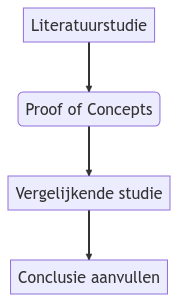
\includegraphics[width=4cm]{flowChart4}
\end{center}

%---------- Verwachte resultaten ----------------------------------------------
\bigskip
\section{Verwacht resultaat}%
\label{sec:verwachte_resultaten}
\paragraph{}
Het verwachte resultaat is een werkende extensie/driver die ervoor zorgt dat een webapplicatie MiFare kaarten rechtstreeks in kan lezen in de browser. Met behulp van deze extensie/driver kunnen vervolgens de toegangskaarten of maaltijdcheques worden gescand via de webapplicatie. Dit stelt gebruikers in staat om start- en stoptijden in te voeren of om gebruik te maken van de maaltijdcheques die aan de kaart zijn gekoppeld.

\bigskip
\section{Verwachte conclusies}%
\label{sec:Verwachte_conclusies}
\paragraph{}
Uit deze bachelorproef moet duidelijk blijken dat het mogelijk is om een card reader rechtstreeks te verbinden met een web app vanuit de browser. De Proof of Concept zal aantonen dat dit haalbaar is en dat MiFare kaarten kunnen worden ingelezen in de web app. Hierdoor kan de web app gebruikmaken van de data op de kaart om toegangskaarten of maaltijdcheques te beheren. Hopelijk vloeit uit dit onderzoek een Proof of Concept die klaar is voor de consument die opzoek is naar een extensie/driver voor het inlezen van chipkaarten in zijn webapplicatie.